\chapter{Task \#15: Cascade Failures - SOC model }
\section{Introduction:}

\textbf{Self-Organized Criticality} (SOC) is an approach adopted to explain the emergence of power-law distributions in natural phenomena. 
In physics, criticality is associated to systems near phase transitions, that live between two distinct regimes, 
and at this critical point, the emergence of power-laws occurs.\\
\noindent In SOC, systems are believed to organize themselves naturally into critical states, following internal feedback mechanisms and without external invervention.
\\
\noindent In this report, we analyze the SOC behavior associated to the Sandpile Model.

\noindent In the \textbf{Sandpile Model}, we consider networks with an associated load variable, that accounts for any sort of stress that can be observed in real applications. 
A given node in the network stays functional, as long as its load doesn't go above a given threshold: its \textit{capacity}. 
Load is assigned randomly to nodes in the network, and when the capacity of a node is overcame, we have a failure in the node, and its load is redistributed according to some chosen rules. 
A dissipative factor is added to load tranfers, to avoid excessive accumulation of load across the network.

\noindent We use single-layer networks\footnote{ Following the works \cite{doi:10.1143/JPSJ.64.327} and \cite{PhysRevLett.91.148701}.} and two-layer networks\footnote{ Following \cite{doi:10.1073/pnas.1110586109}.}, where the first ones are used to examine the basic properties of cascade failures, 
and the second offers a more robust study of interconnected systems, such as real power grids.

\noindent To analyze the cascades, we assume a tree structure of each avalanche, and using the theory of multiplicative branching processes, we find the analytical predictions for the distributions of the size $s$ of the avalanches and their lifetime $t$
\\
\noindent For the systems studied in this work, the results for the size ($s$) and lifetime ($t$) distributions are:

\begin{gather}
    p(s)\sim s^{-\tau}
    \\
    l(t)\sim t^{-z}
\end{gather}

\begin{table}[htbp]
    \centering
    \begin{tabular}{lc|c|c}
        \toprule
        \textbf{Network} && $\tau$ & $z$ \\
        \midrule
        Random && $3/2$ & $2$ \\
        \hline
        & $2<\gamma<3$ & $\frac{\gamma}{\gamma-1}$ & $\frac{\gamma-1}{\gamma-2}$ \\
        Scale-free ($\gamma$) & $\gamma=3$& $3/2^*$ & $2^*$\\
        & $\gamma\ge3$ & $3/2$ & $2$\\
        \hline
        Two-layer\tablefootnote{Sparsely interconnected network, where each layer $i$ has nodes with fixed degree $k_i$.} & - & - \\
        \bottomrule
    \end{tabular}
    \caption{Analytical predictions for avalanche distributions. \\
    $^*$with logarithmic corrections.}
    \label{tab:analytical_res}
\end{table}




\section{Analysis} 

\noindent In this work, we first consider the Sandpile Model with simple degree distributions, in particular, following the works \cite{doi:10.1143/JPSJ.64.327} and \cite{PhysRevLett.91.148701}, we use the distributions:
\begin{itemize}  
    \item Gaussian: $k \sim \mathcal{N}(\mu=20,\sigma=8)$
    \item Uniform: $k\sim\text{Uniform}(k_{min}=4,k_{max}=36)$
    \item Power Law (Scale Free): $k\sim k^{-\gamma}$ with $\gamma\in\{2.01,2.2,2.4,2.6,2.8,3.0,5.0\}$
\end{itemize}

\noindent Every network includes $N=10^5$ nodes, and the results are the averages of $30$ different iterations.
The dissipation is carried by dissipative nodes ($0.1\%$ of the total) in the random networks, which transfer load outside of the network once toppled; we use a dissipation probability $f=0.001$ on the scale free network, 
which is the probability of every load transfer to not happen, dissipating the load.

\begin{figure}[htbp]
    \centering
    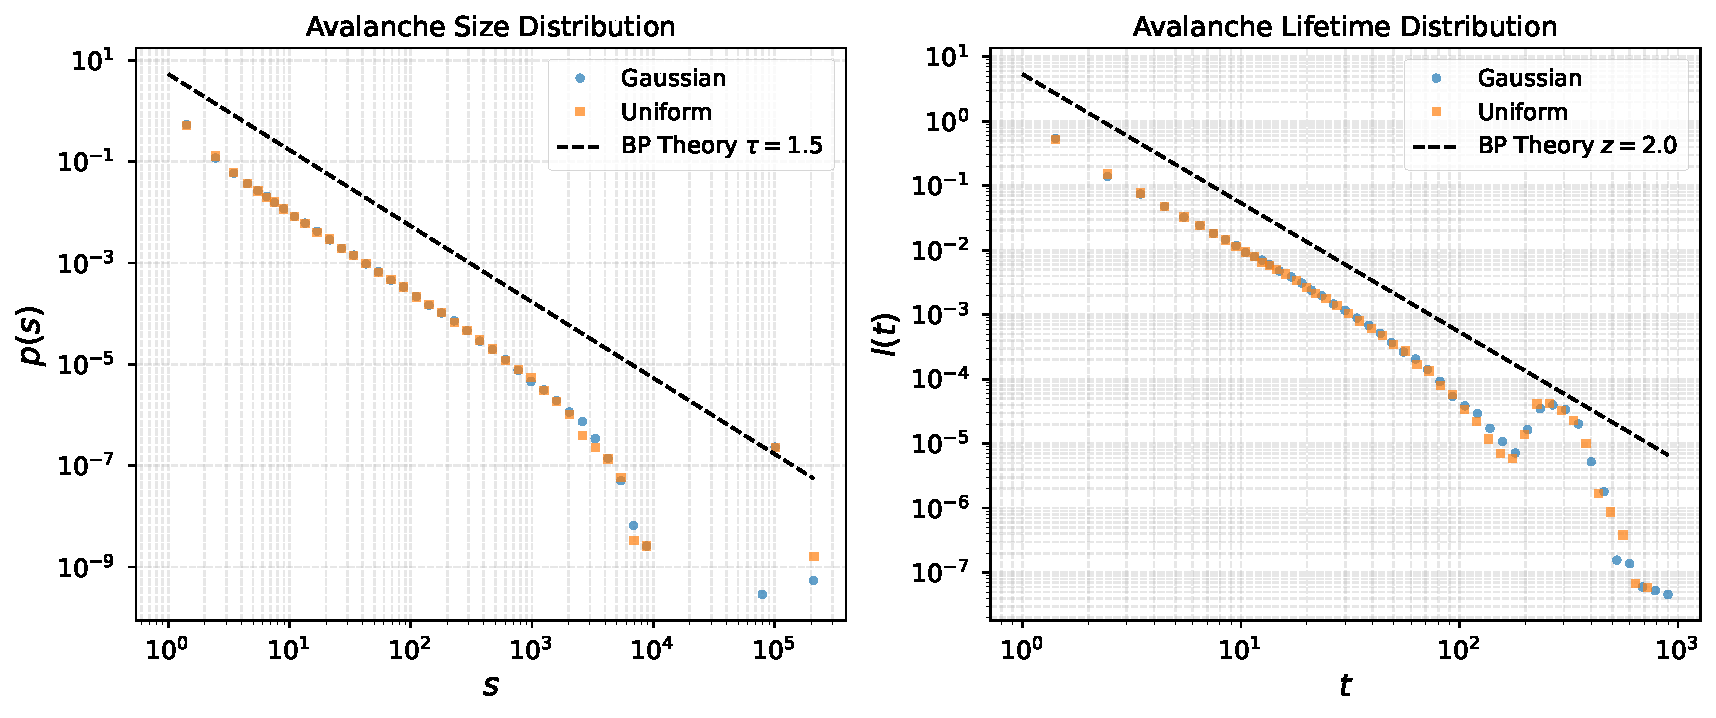
\includegraphics[width=0.9\textwidth]{./figures/task_15/task_15_part1.pdf}
    \caption{Avalanche size ($s$) and lifetime ($t$) distributions for the SOC sandpile model on Gaussian and Uniform networks.}
\end{figure}
\begin{figure}[htbp]
    \centering
    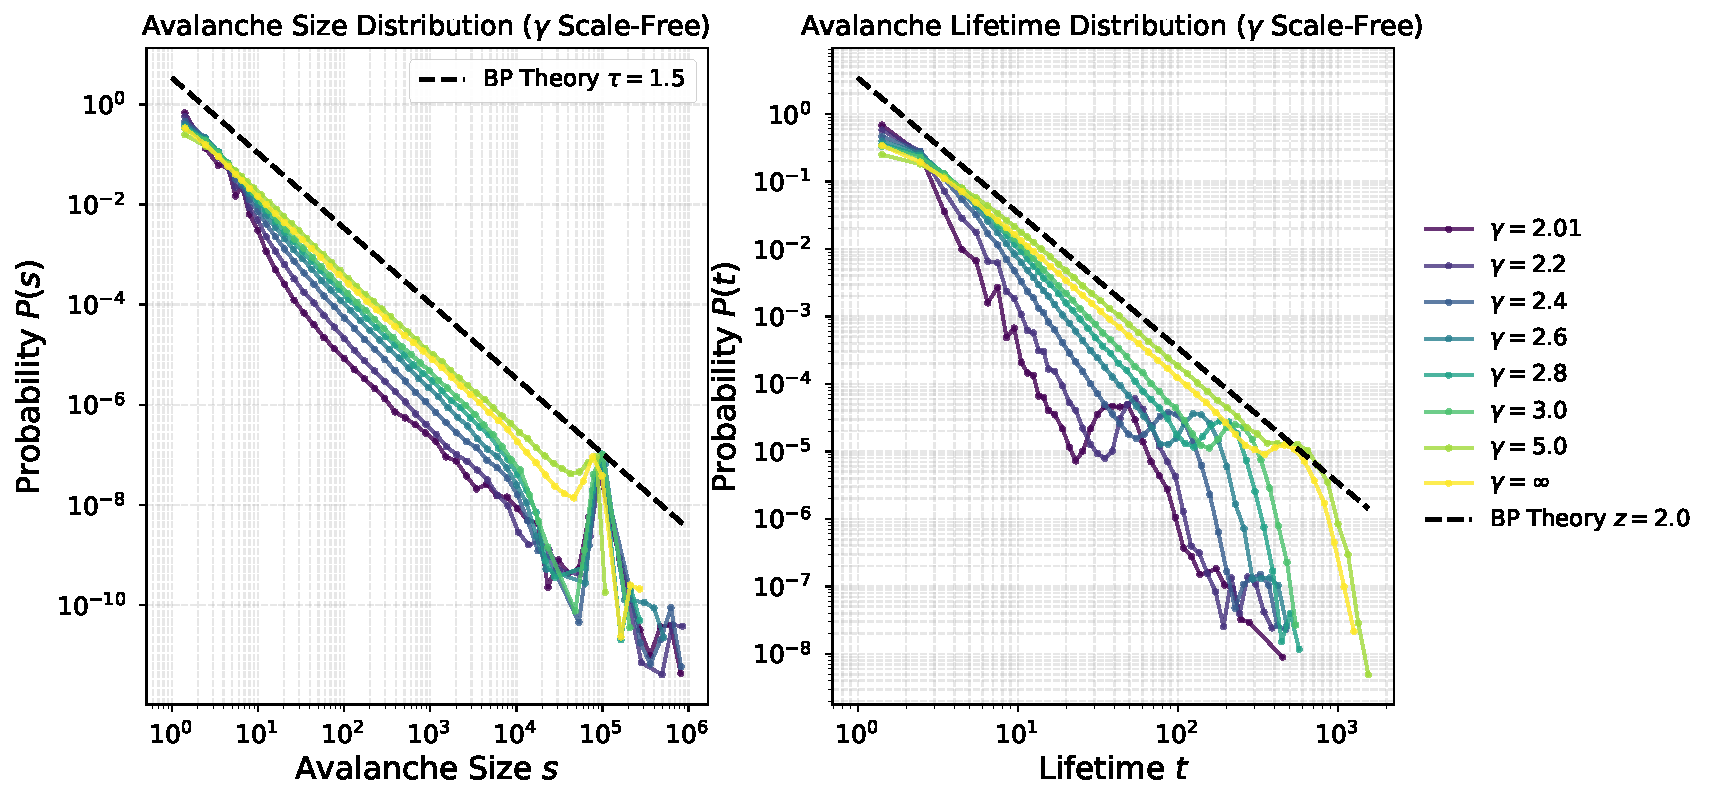
\includegraphics[width=0.9\textwidth]{./figures/task_15/task_15_part2.pdf}
    \caption{Avalanche size ($s$) and lifetime ($t$) distributions for the SOC sandpile model on Scale-Free networks.}
\end{figure}

\noindent From the log-binned distributions we estimate the exponents of the scaling regimes, and compare them with the analytical predictions of multiplicative branching processes. The fits are performed with weighted least squares on the \emph{plateau} of each distribution: a window of fixed logarithmic span is slid across the data and the straightest portion (minimum local-slope variance) is selected, after excluding the small-size cut-off and the noisy tail of the distributions. The resulting scaling ranges are reported in Table~\ref{tab:fit_ranges}.

\begin{table}[htbp]
    \centering
    \begin{tabular}{lc|cc|cc}
        \toprule
        \textbf{Network} && \multicolumn{2}{c|}{$\tau$} & \multicolumn{2}{c}{$z$} \\
        & & theory & fit & theory & fit \\
        \midrule
        Gaussian && 1.50 & 1.55 $\pm$ 0.02 & 2.00 & 1.95 $\pm$ 0.01 \\
        Uniform && 1.50 & 1.57 $\pm$ 0.02 & 2.00 & 1.94 $\pm$ 0.01 \\
        $\gamma = 2.01$ && 1.99 & 1.74 $\pm$ 0.03 & 101.00 & 5.58 $\pm$ 0.21 \\
        $\gamma = 2.2$ && 1.83 & 1.77 $\pm$ 0.01 & 6.00 & 3.91 $\pm$ 0.14 \\
        $\gamma = 2.4$ && 1.71 & 1.78 $\pm$ 0.02 & 3.50 & 3.48 $\pm$ 0.03 \\
        $\gamma = 2.6$ && 1.62 & 1.69 $\pm$ 0.02 & 2.67 & 2.98 $\pm$ 0.01 \\
        $\gamma = 2.8$ && 1.56 & 1.72 $\pm$ 0.01 & 2.25 & 2.71 $\pm$ 0.01 \\
        $\gamma = 3.0$ && 1.50 & 1.69 $\pm$ 0.01 & 2.00 & 2.51 $\pm$ 0.01 \\
        $\gamma = 5.0$ && 1.50 & 1.66 $\pm$ 0.00 & 2.00 & 2.01 $\pm$ 0.01 \\
        $\gamma = \infty$ && 1.50 & 1.67 $\pm$ 0.00 & 2.00 & 2.10 $\pm$ 0.01 \\
        \bottomrule
    \end{tabular}
    \caption{Fitted avalanche-size ($\tau$) and lifetime ($z$) exponents vs multiplicative branching-process predictions.
    Fits are performed on the plateau of each log-binned distribution; the corresponding scaling ranges are listed in Table~\ref{tab:fit_ranges}.}
    \label{tab:fitted_exponents}
\end{table}

\begin{table}[htbp]
    \centering
    \begin{tabular}{lc|cc|cc}
        \toprule
        \textbf{Network} && \multicolumn{2}{c|}{$s$} & \multicolumn{2}{c}{$t$} \\
        & & min & max & min & max \\
        \midrule
        Gaussian && 27 & 1e+02 & 5 & 3e+01 \\
        Uniform && 21 & 1e+02 & 4 & 3e+01 \\
        $\gamma = 2.01$ && 77 & 4e+02 & 54 & 1e+02 \\
        $\gamma = 2.2$ && 173 & 9e+02 & 4 & 3e+01 \\
        $\gamma = 2.4$ && 132 & 7e+02 & 6 & 4e+01 \\
        $\gamma = 2.6$ && 259 & 2e+03 & 8 & 5e+01 \\
        $\gamma = 2.8$ && 87 & 5e+02 & 10 & 6e+01 \\
        $\gamma = 3.0$ && 69 & 4e+02 & 10 & 6e+01 \\
        $\gamma = 5.0$ && 16 & 9e+01 & 29 & 2e+02 \\
        $\gamma = \infty$ && 10 & 5e+01 & 9 & 6e+01 \\
        \bottomrule
    \end{tabular}
    \caption{Scaling ranges used for the exponent fits of Table~\ref{tab:fitted_exponents}.}
    \label{tab:fit_ranges}
\end{table}

\noindent The fitted exponents are in good agreement with the multiplicative branching process predictions: the lifetime exponent matches $z = 2$ within statistical error on the random networks, and the size exponent is only slightly above the mean-field value $\tau = 3/2$ (a finite-size effect already visible in the plateau of the local slopes).
For the scale-free networks the observed exponents decrease with $\gamma$ as predicted, although for $\gamma \lesssim 2.6$ the fitted $\tau$ and $z$ remain below the theoretical values; for $\gamma$ close to $2$ the theoretical lifetime exponent diverges as $z = (\gamma-1)/(\gamma-2)$, which is not attainable in finite networks, so the comparison there is indicative rather than quantitative.

\section{Interconnected Networks}

\noindent We conclude the analysis by studying how interconnectivity between two networks affects cascading failures, following the work of Brummitt \emph{et al.}\cite{doi:10.1073/pnas.1110586109}. 
Real power grids are sparsely interconnected and possess narrow degree distributions; to model this we consider two independent random 3-regular graphs, each with $N=2\times10^3$ nodes, coupled by a \emph{Bernoulli interconnection}: each node of either network independently receives one additional external edge stub with probability $p$ (and none with probability $1-p$). 
The external stubs of the two networks are then matched uniformly at random, so that both networks have the same number of interconnections. 
We denote this topology by $R(3)\text{-}B(p)\text{-}R(3)$; nodes therefore have degree $3$ (with probability $1-p$) or $4$ (with probability $p$), and the threshold of each node is its total degree, as before.

\noindent We run the sandpile dynamics with dissipation rate $f=0.01$, chosen so that the largest cascades topple almost the entire network, dropping $2\times10^6$ grains per realization (after a $20\%$ transient) on $30$ independent realizations for each of the $10$ values of $p$ in $[0.001,\,0.5]$, concentrating on small $p$ as in the reference work.
For every avalanche we record the number of topplings $T_a$ and $T_b$ caused in each network, together with the network in which the cascade began.
A cascade is deemed \emph{large} if it topples at least half of the nodes of network $a$, i.e. $T_a>1000$.

\begin{figure}[htbp]
    \centering
    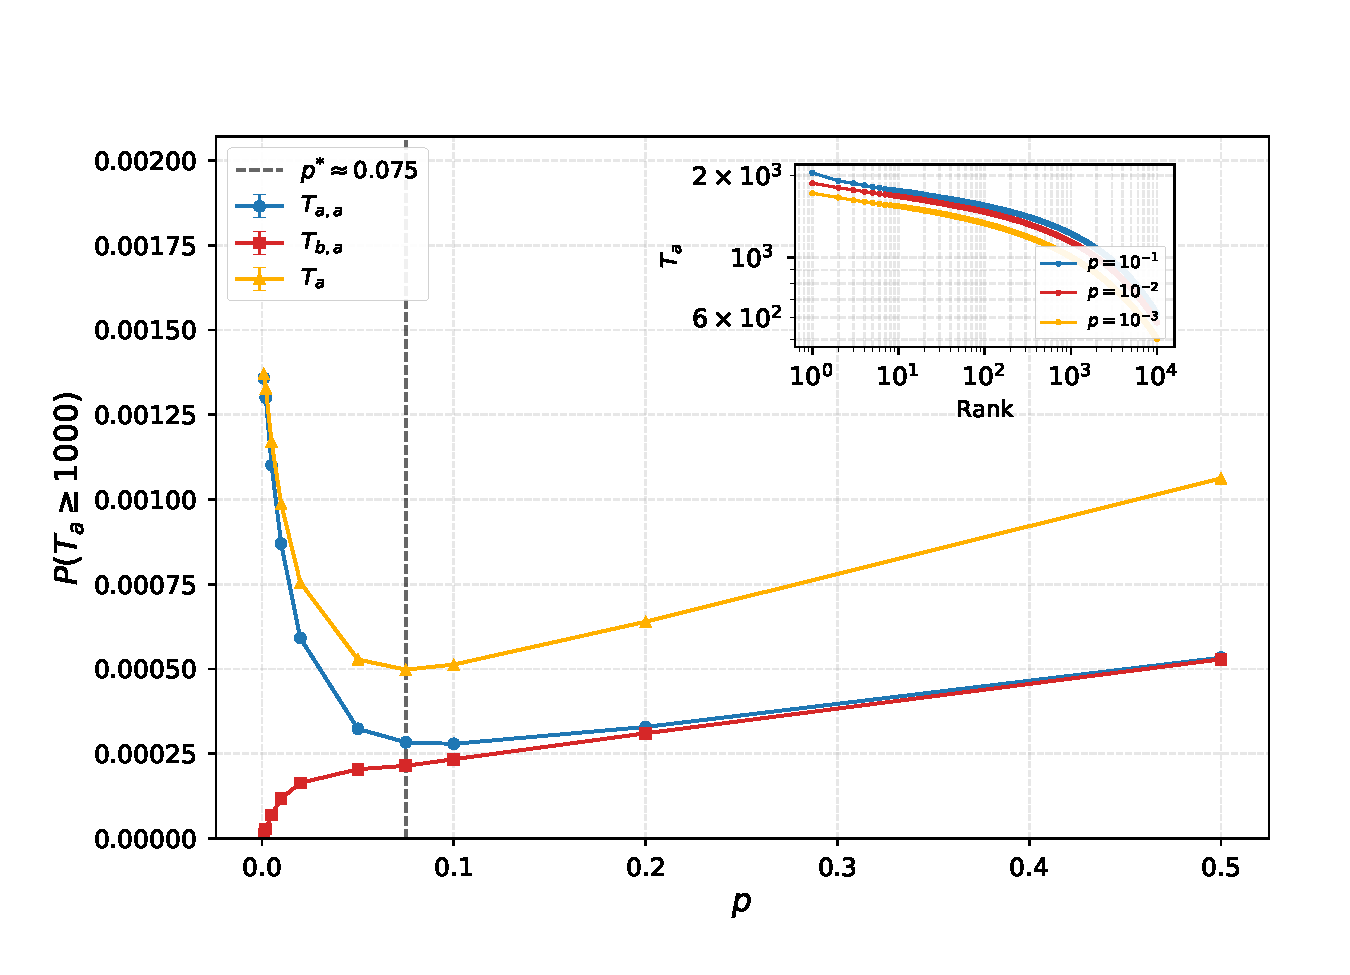
\includegraphics[width=0.85\textwidth]{./figures/task_15/task_15_part3_fig4.pdf}
    \caption{Probability of a large avalanche ($T_a>1000$) in network $a$ as a function of the interconnectivity $p$ on $R(3)\text{-}B(p)\text{-}R(3)$ networks ($N=2\times10^3$/network, $f=0.01$, $2\times10^6$ grains, 30 iterations).
    Large cascades \emph{beginning} in $a$ (blue) first decrease and then increase with $p$, whereas cascades beginning in $b$ and toppling most of $a$ (red) become monotonically more likely.
    Their average (gold) has a stable minimum at $p^{*}\approx0.075$. 
    Inset: log-log rank-size plots of the $10^4$ largest values of $T_a$ for $p=10^{-1},10^{-2},10^{-3}$, showing the suppression of the largest local cascades as interconnectivity is initially increased.}
    \label{fig:part3_fig4}
\end{figure}

\noindent Figure~\ref{fig:part3_fig4} shows the central result: adding a few interconnections between the networks is \emph{locally stabilizing} -- the probability of a large avalanche in $a$ initially drops with $p$, because excess load is absorbed by the neighboring network, which acts as a reservoir.
However, beyond a critical amount of interconnectivity the probability rises again, for two reasons: interconnections open pathways for network $b$ to \emph{inflict} large cascades onto $a$ (the red curve only ever increases), and every added interconnection augments the total capacity and average load of the system, fueling larger cascades.
The two effects balance at $p^{*}\approx0.075\pm0.01$, where the probability of a large avalanche in $a$ is minimized; this value is stable across the range of cutoffs $C\in[400,1500]$.

\begin{figure}[htbp]
    \centering
    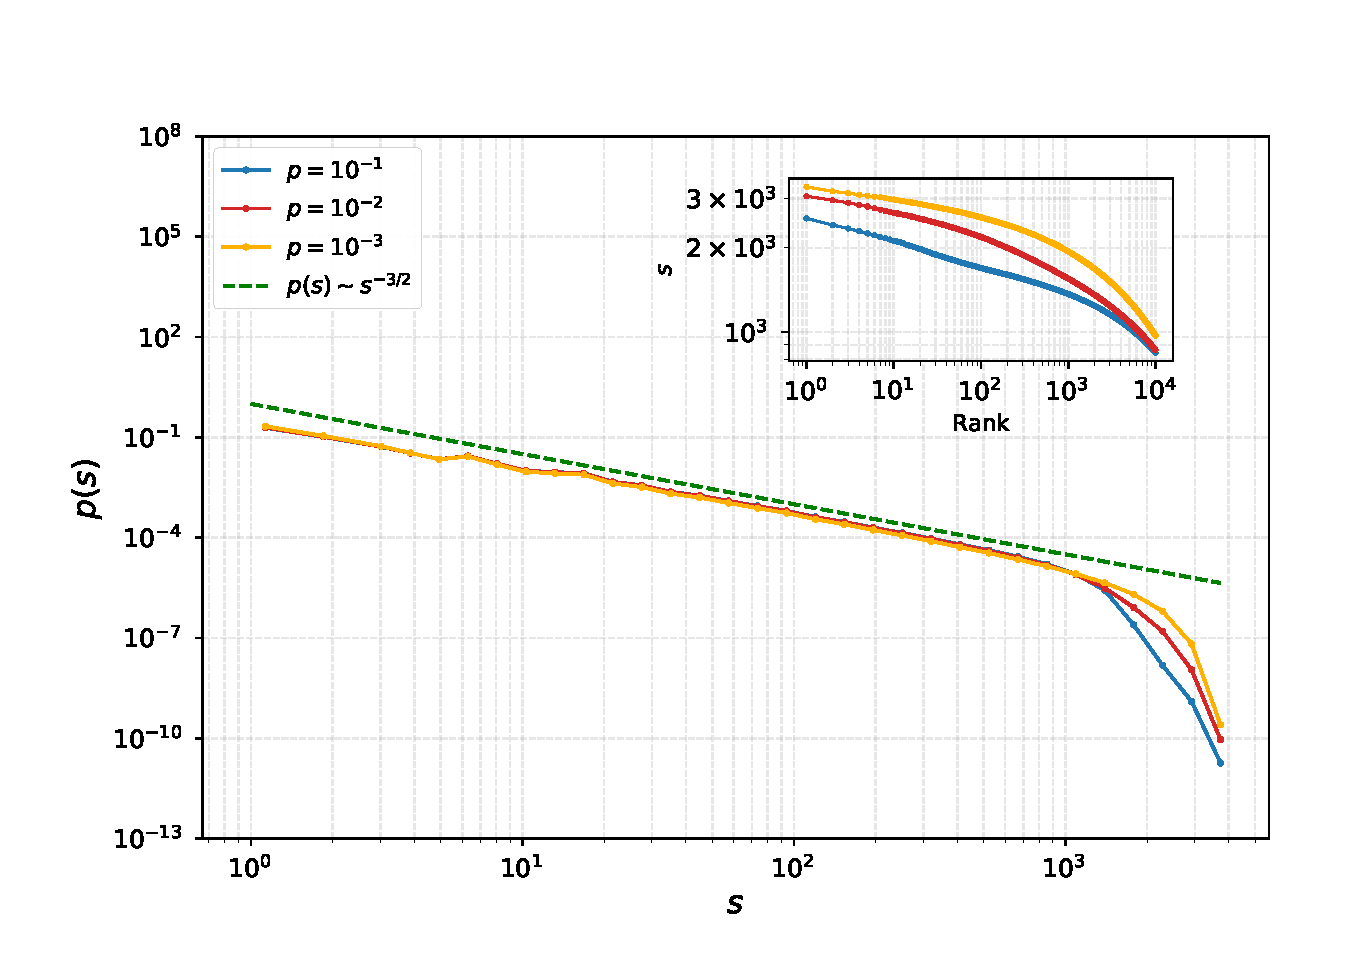
\includegraphics[width=0.85\textwidth]{./figures/task_15/task_15_part3_fig5.pdf}
    \caption{Total avalanche size distribution $s(t)$ (topplings in both networks) on $R(3)\text{-}B(p)\text{-}R(3)$ for $p=10^{-3},10^{-2},10^{-1}$, in log-log.
    The green dashed line is the mean-field prediction $s(t)\sim t^{-3/2}$ obtained when both networks are viewed as a single system.
    Inset: log-log rank-size plot of the $10^4$ largest global cascades, showing that increasing $p$ enlarges the largest cascades of the whole system by an amount on the order of the additional interconnections.}
    \label{fig:part3_fig5}
\end{figure}

\noindent The locally stabilizing effect is specific to each individual network; the collection of networks viewed as one system is instead \emph{globally destabilized} by interconnectivity.
Figure~\ref{fig:part3_fig5} shows that the total avalanche size distribution $s(t)$ (not distinguishing between topplings in $a$ and $b$) develops a longer tail as $p$ grows, and the inset confirms that the largest global cascades become larger with $p$: while a single network benefits from interconnectivity, the whole system suffers larger cascades.

\begin{figure}[htbp]
    \centering
    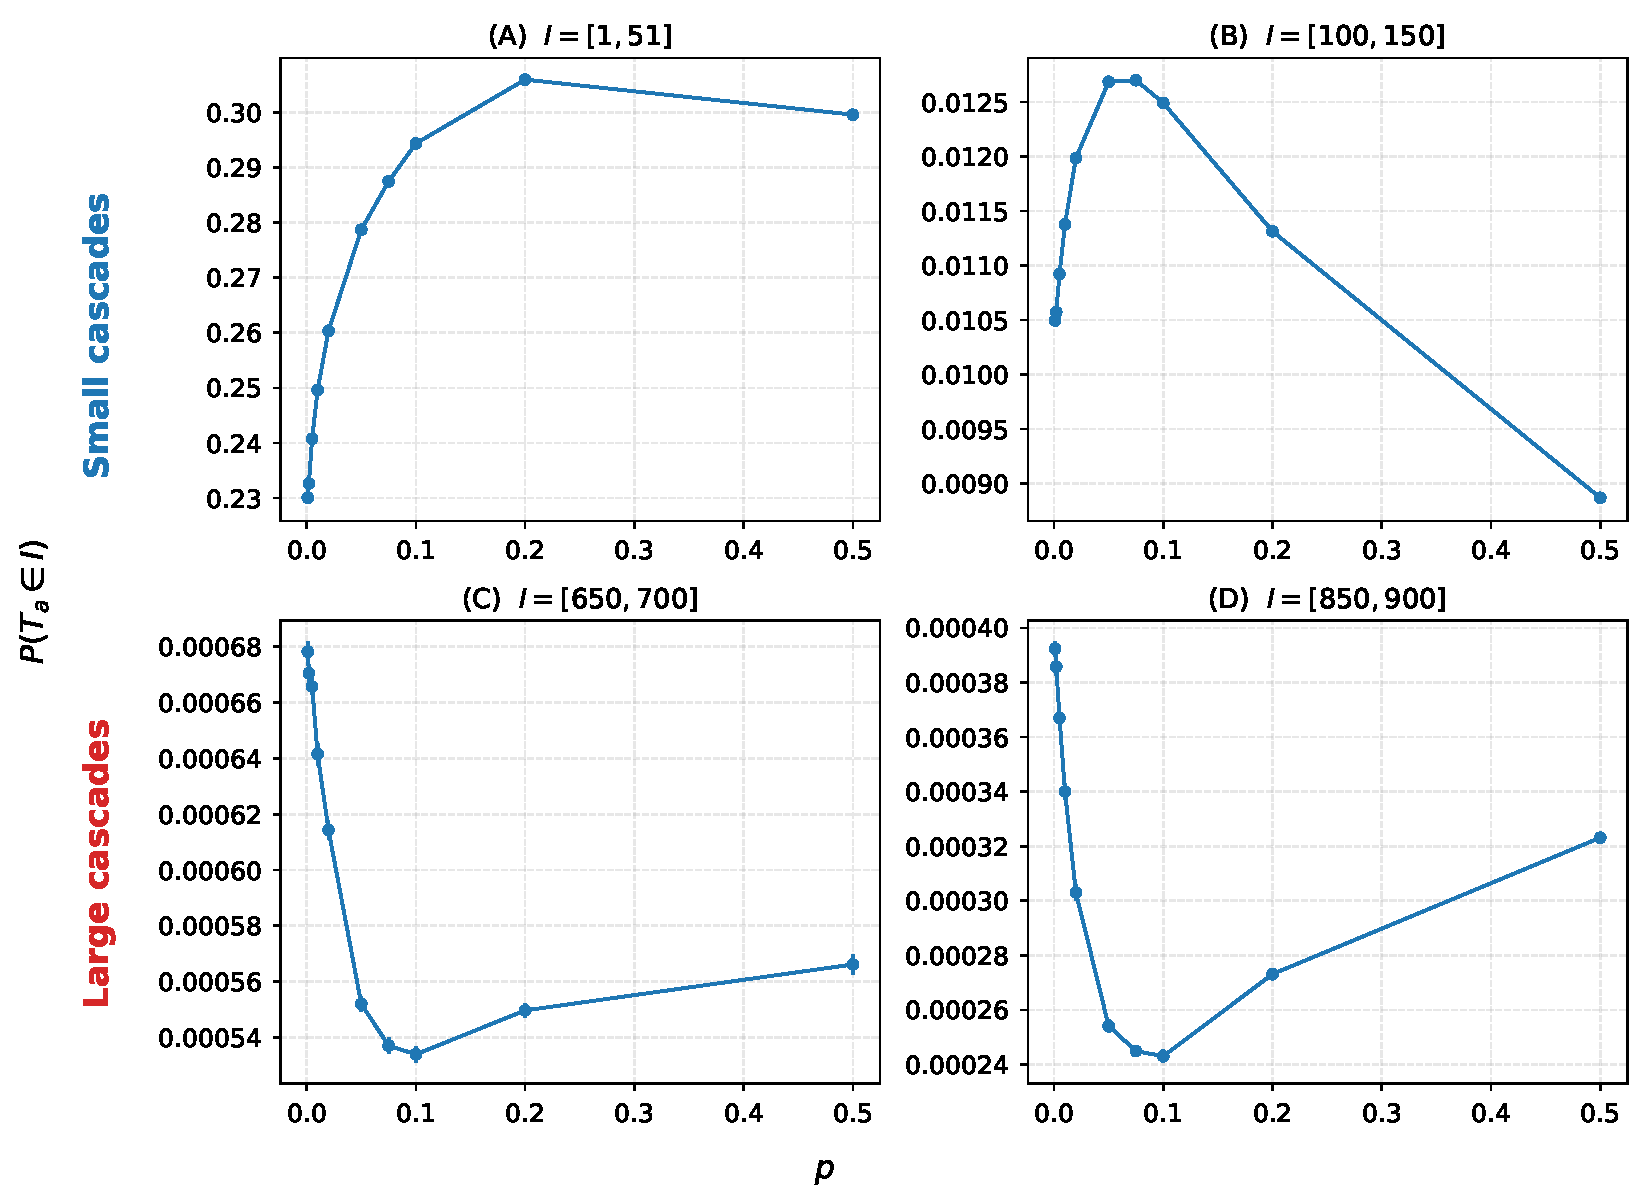
\includegraphics[width=0.85\textwidth]{./figures/task_15/task_15_part3_fig6.pdf}
    \caption{Probability that a cascade in network $a$ has total size $T_a$ within each of four windows, as a function of $p$ on $R(3)\text{-}B(p)\text{-}R(3)$.
    Small cascades (A) become more likely with $p$; intermediate cascades (B) peak at an unstable critical point near $p^{*}\approx0.075$; the largest cascades (C, D) are minimized at the stable equilibrium $p^{*}\approx0.075$.
    Tuning the interconnectivity to suppress one range of cascade sizes amplifies the others.}
    \label{fig:part3_fig6}
\end{figure}

\noindent Figure~\ref{fig:part3_fig6} shows that the effect of interconnectivity depends on the size of the cascade considered: small cascades ($1\le T_a\le51$) are always favored by larger $p$, intermediate cascades ($100\le T_a\le150$) occur most frequently at an \emph{unstable} critical point around $p^{*}\approx0.075$, while the largest cascades ($650\le T_a\le700$ and $850\le T_a\le900$) are suppressed at the \emph{stable} equilibrium $p^{*}\approx0.075$.
A network cannot simultaneously mitigate all cascade sizes: interconnectivity that minimizes the largest cascades amplifies the intermediate ones, and vice versa.
These results are in qualitative agreement with the multitype branching process analysis of Ref.~\cite{doi:10.1073/pnas.1110586109}, which predicts the average number of topplings in the same and in the neighboring network at the next time step to vary as $\langle u_a\rangle_a = 1 - p/(1+z_a)$ and $\langle u_a\rangle_b = p/(1+z_b)$, respectively: the branching process remains critical (leading eigenvalue $1$) for every $p$, yet load is increasingly diverted from one network to the other as $p$ grows.
\newpage